\chapter{Deep Learning Background} \label{chapter:deep}
  \section{Introduction}
    pass
  \section{Model Components}
    \subsection{Artificial Neural Networks}
  An artificial neuron is a function which takes in a vector of inputs, computes their
  weighted sum and applies a non-linearity as follows:
  \begin{equation}
    a(\mathbf{x}) = \sigma \left ( \sum_{i=1}^N w_ix_i + b \right )
  \end{equation}
  Here $\sigma$ is a scalar function, $w_i$ is a scalar weight and $b$ is its bias. $N$ is the size of the input and weight vector.
  These neurons can be combined into layered networks to construct artificial neural networks.
  The weights $w$ can then be rewritten as matrices $\mathbf{W}$ which define how
  activations from one layer are transferred to the next\footnote{Note: when a vector
  is put into a scalar function it is assumed that it acts on each element of
  the vector. The only exception is with the softmax.}.
  \begin{equation}
    \mathbf{a}(\mathbf{x}) = \mathbf{\sigma} \left ( \mathbf{W}\mathbf{x} + \mathbf{b} \right ) \label{eq:softmax}
  \end{equation}

  Popular activation functions include:
  \begin{multicols}{2}


    \begin{equation}
      \text{The sigmoid:}\quad
      \sigma (x) = \frac{1}{1-e^{-x}} \label{eq:sigmoid}
    \end{equation}


    \begin{equation}
      \text{The ReLU:}\quad
      \sigma(x) =
      \begin{cases}
        x & x\geq 0 \\
        0 & x < 0
      \end{cases}
    \end{equation}


    \begin{equation}
      \text{Hyperbolic tan:}\quad
      \sigma(x)=\frac{e^x - e^{-x}}{e^x + e^{-x}}
    \end{equation}


    \begin{equation}
      \text{The softmax:}\quad
      \sigma(\mathbf{x})_j = \frac{e^{x_j}}{\sum_i e^{x_i}}
    \end{equation}


  \end{multicols}

  \begin{figure} \label{disfagraph}
    \center
    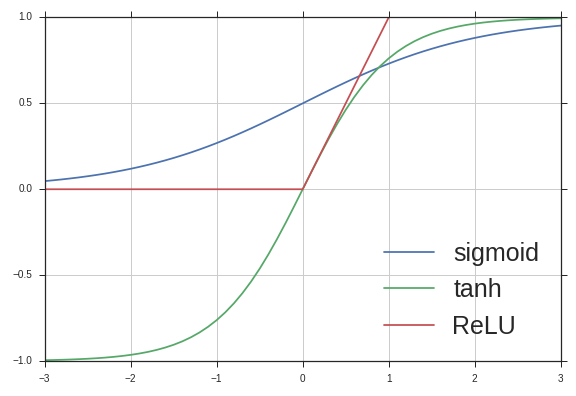
\includegraphics[width=.5\textwidth]{../graphs/actfuncs.pdf}
    \caption{Comparison of common activation functions for neural networks}
  \end{figure}



  An $N$ layer network can
  then be thought of as a function with a recursive structure (these are also known as fully connected layers):
  \begin{equation}
    \mathbf{y} = \mathbf{a}_{N}(\mathbf{a}_{l-1}(...\mathbf{a}_1(\mathbf{x})...))
  \end{equation}
  Now assuming there exists a set of $\tilde{\mathbf{x}}$ and $\tilde{\mathbf{y}}$ which make
  up a training data set, these could be sets of images and labels, then a cost function
  to optimise can be defined:
  \begin{equation}
    J(\tilde{\mathbf{x}},\tilde{\mathbf{y}}) = \frac{1}{N}\left |\mathbf{y}(\tilde{\mathbf{x}})-\tilde{\mathbf{y}}\right | ^2
  \end{equation}
  this is called the least mean squared error, another popular cost function is
  the cross entropy:
  \begin{equation}
    J(\tilde{\mathbf{x}},\tilde{\mathbf{y}}) = -\frac{1}{N}\tilde{\mathbf{y}}\cdot\log(\mathbf{y}(\tilde{\mathbf{x}}))
  \end{equation}

  The derivative of these cost functions can then be computed in order to minimise it.
  The simplest way is to do this is per training example, however stochastic gradient
  descent\cite{Amari1993} has emerged as a superior method. Simply put it computes the gradient with respect
  to many randomly drawn samples, it has the advantage of following a smoother path
  towards the local minimum.
  \subsection{Convolutional Layers}
  A convolutional layer is a generalisation of simple fully connected layers described
  above. It consists of a set of $K$ filters of size $m\times m$, which are applied to the input to produce
  a set of $K$ outputs. The filters are applied with a 2D convolution.


  To describe them, firstly assume that any vector described in the previous section
  can also be rewritten as a matrix, i.e $\mathbf{x} \in \mathbb{R}^{n}
  \rightarrow \mathbf{x} \in \mathbb{R}^{N \times M} \quad NM=n$, in practice this is made
  easy by using numbers which factorise well.

  Then the following equation describes the output of a convolutional layer:
  \begin{equation} \label{CNN}
    \mathbf{a}(\mathbf{x})_{ijk} = \sigma \left ( \sum_{a=0}^{m-1}\sum_{b=0}^{m-1}(w_{abk}x_{(i+a)(j+b)k}) + b_k \right )
  \end{equation}
  Here $i,j$  denote row, column indices for the matrix (image) $\mathbf{x}$, $k$ is the filter index, $w_{abk}$
  gives the filter element and $b_k$ is the bias for that filter. This is done for all $K$ filters.

  One issue is how to deal with indices which are out of bounds, SAME padding can be used which sets out of bounds
  elements to zero and so preserves the image size or VALID can be used, this keeps the filter within the bounds of the
  image and hence the output is of a smaller dimension. Lastly a stride greater than 1 can be incorporated into equation
  \ref{CNN} meaning that $\mathbf{a}$ is only computed for a fraction of indices $i,j$.
  % \begin{equation}
  % 	C : \mathbb{R}^{n\times m \times p \times l} \rightarrow \mathbb{R}^{N\times M \times l \times K}
  % \end{equation}
  %con%
  \subsection{Max Pooling Layers}
  A max pooling layer simply splits its input into a set of sections and extracts
  the highest value from each. It is a simple but effective method to down sample
  an image, it helps to keep the computational overhead of these algorithms
  down. However a recent trend \cite{Springenberg2015} has emerged where max pooling
  layers are not used, instead a convolutional layer with a large stride accomplishes
  the same amount of down-sampling.
    \subsection{Cost Functions}
      pass
    \subsection{Training algorithms}
      pass
      \subsubsection{Gradient Descent}
        pass
      \subsubsection{Stochastic Gradient Descent}
        pass
      \subsubsection{Adam}
        pass
      \subsubsection{Comparison}
        pass
    \subsection{Regularisers}
      pass
    \subsection{Dropout Layers} \label{sec:dropout}
      A layer with dropout applied to it randomly turns neurons off, making it more
      difficult for the network to overfit data. There is a dropout probability
      which determines how often neurons are disabled, it is typically under 20\%
    \subsection{Autoencoders}
      An autoencoder is at its bare minimum a artificial neural network which tries
      to reproduce its input as accurately as possible. So the cost function for the mean squared error becomes:

      \begin{equation} \label{eq:autoencoder_cost}
        J(\tilde{\mathbf{x}},\tilde{\mathbf{y}}) = \frac{1}{N}\left |\mathbf{y}(\tilde{\mathbf{x}})-\tilde{\mathbf{x}}\right | ^2
      \end{equation}

      Constraints are
      placed on the network so that it has to learn to compress the input, the following
      are popular constraints that may be used:
      \begin{itemize}
        \item Few neurons in the hidden layers
        \item Sparsity: the average activation of the neurons can be kept under a
        threshold, typically a small value close to zero \cite{autong}
        \item Noise may be added to the input, this makes the network more likely
        to learn general features.
      \end{itemize}
      Lastly there are Variational Autoencoders which combine ideas from Bayesian inference
      to create networks which can not only reconstruct their input but also act as a
      distribution which can be sampled from, allowing for the generation of new samples \cite{Kingma2013}.

    \subsection{Stacked Autoencoder}
      A stacked autoencoder is typically used for pre-training a network for a classification task.
      Instead of training the whole structure at once, each layer is trained as the last hidden
      layer of some temporary autoencoder. It has been shown that this can improve classification performance \cite{stacks}.
    \subsection{Convolutional Autoencoder}
      A convolutional autoencoder works in the same way as a standard autoencoder, however
      undoing the max pooling presents a problem, as a max pooling layer throws away
      information, its inverse will never be exact. The following strategies have been
      used with success:
      \begin{itemize}
        \item Replacing each entry with an $n \times n$ matrix filled with the original
        entry.
        \item Replacing each entry with an  $n\times n$  matrix with
        the original entry in the upper left and the other squares set to 0. \cite{Dosovitskiy2015}
      \end{itemize}

      Other than that all other elements have very straightforward inverses and hence
      a convolutional autoencoder can be constructed.
    \subsection{LRN}
      pass
  \section{Model Evaluation}
    With any kind of classification model it is crucial to be able to evaluate its
    performance in a standard and reproducible way. For the problem of classifying
    AUs the simplest case is to split the problem into a set of $n_C$ decision problems
    where $n_C$ is the number of distinct classes. Now the problem is reduced to
    evaluating the performance of a binary classifier.


    Naively the first metric one might use for measuring the performance of a classifier
    might be the accuracy, this is good for datasets which are evenly balanced however
    the datasets of interest in this report typically have many more negative labels than postive labels.
    A classifier that simply labels all examples negative might then get a very high accuracy. This motivates
    defining a matrix called the confusion matrix whose elements express accuracy from various angles.
    For a binary problem the confusion matrix is defined as:
    \begin{equation}
      C =
      \begin{pmatrix}
        TP & FN\\
        FP & TN
      \end{pmatrix}
    \end{equation}
    Where $TP$ is the number of true positives, $FN$ is the number of false negatives
    , $FP$ is the number of true positives and $TN$ is the number of true negatives.
    In a perfect classification, this matrix would have $FP=FN=0$, however this is
    difficult to achieve
    and we can define quantities to measure how close to this ideal we are. Note we
    only define the binary case here, the more general confusion matrix for multiple
    classes can easily be defined but is not relevant here.
    \begin{equation}
      \text{Recall} = \frac{TP}{TP+FN}
    \end{equation}
    \begin{equation}
      \text{Precision} = \frac{TP}{TP+FP}
    \end{equation}
    \begin{equation}
      \text{F1} = 2 \cdot \frac{\text{Recall} \cdot \text{Precision}}{\text{Recall} + \text{Precision}}
    \end{equation}

    Hence recall is decreased by false negatives, i.e not being able to recall the class
    when presented with it. Precision is decreased by false positives i.e stating the class
    is present when it is not. Both measures describe a different aspect of the accruacy. This
    motivates defining the F1 score which is the harmonic mean between the precision and recall
    (the harmonic mean is used to ensure that case where $R=1$ and $P=0$ R,P being Recall and Precision, gives
    a very low score  as achieving $R=1$ is trivial.) The F1 is the quantity this report will seek to maximise and use to compare
    results with the literature.

    Another useful measure is the area under the Receiver operating characteristic (ROC) curve.
    As neural networks output a number between 0 and 1, a threshold must be chosen to signify
    when the network declares a class present. By varying this threshold a series of true positive and false positive rate points
    can be generated, this is the ROC curve. The area under this is ideally 1 and in the worst case 0.5 (TP = FP), hence this is
    another measure of classification accuracy that is invariant to the chosen threshold.

    \begin{table}[]
      \centering \caption{A simple qualitative illustration of what a ROC score means for a classifier.
      Note: It is typically only in strange cases that $ROC< 0.5$ but is possible.} \label{my-label}
      \begin{tabular}{rl}
        \hline
        Range & Classifier quailty \\ \hline
        $0 \leq ROC \leq 0.6$   & Fail               \\
        $0.6 \leq ROC    < 0.7$   & Poor               \\
        $0.7 \leq ROC    < 0.8$   & Fair               \\
        $0.8 \leq ROC    < 0.9$   & Good               \\
        $0.9 \leq ROC \leq 1.0$   & Great              \\ \hline
      \end{tabular}
    \end{table}



    % if roc < 0.6:
    %     return 'fail'
    % elif roc < 0.7:
    %     return 'poor'
    % elif roc < 0.8:
    %     return 'fair'
    % elif roc < 0.9:
    %     return 'good'
    % else:
    %     return 'great'
